\section{\index{Backend Architecture}Backend Architecture Specifications}

\begin{itemize}
    \item There are $n$ buses: $0, 1, 2, \ldots n-1$
    \item There are $m$ stops: $0, 1, 2, \ldots m-1$  ($0$: first stop, $m-1$: last stop)
    \item We have to synchronize the \textit{\gls{24-hour clock}} at each stop
    \item In this system, all bus shifts end at the starting stop, i.e. the bus shift ends when the bus is back at the $0$\textsuperscript{th} stop. The sequence followed in a shift is \\
          {\bfseries $0$ $\to$ $1$ $\to$ $2$ $\to$ $3$ $\to$ \ldots $\to$ $m-2$ $\to$ $m-1$ $\to$ $m-2$ $\to$ \ldots$\to$ $3$ $\to$ $2$ $\to$ $1$ $\to$ $0$}\\
\end{itemize}

\begin{figure}[H]
        \centering
        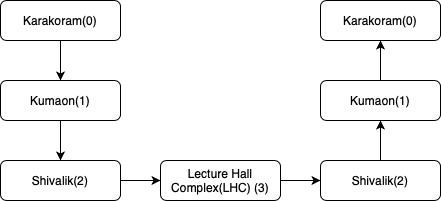
\includegraphics[width=0.7\textwidth]
        {./Files/Images/Flowchart.png}
        \caption{\textbf{Example for m = 4}} % Add a caption
    \end{figure}
    
\subsection{Data Storage and Timing Estimates}
\subsubsection{Over the Network}

\begin{enumerate}

\item Maintain the \textbf{Arrival}\textsubscript{mxn} matrix : Element $(i, j)$ stores the arrival time of $j$\textsuperscript{th} bus at the $i$\textsuperscript{th} stop
\item Maintain the \textbf{Departure}\textsubscript{mxn} matrix : Element $(i, j)$ stores the departure time of $j$\textsuperscript{th} bus at the $i$\textsuperscript{th} stop
\item Maintain the \textbf{PassengerWaitingAtStop}\textsubscript{1xm} matrix : Element $(0, j)$ is $x$ where
 \[ x = \begin{cases} \mbox{1} & \mbox{if any passenger is waiting at the j\textsuperscript{th} stop}  \\ \mbox{0} & \mbox{otherwise} \end{cases} \]
\item Maintain the \textbf{Direction}\textsubscript{1xn} matrix : Element (0, j) is x where
 \[ x = \begin{cases} \mbox{0} & \mbox{if $j$\textsuperscript{th} bus is moving towards $0$\textsuperscript{th} stop}  \\ \mbox{1} & \mbox{if $j$\textsuperscript{th} bus is moving towards $m-1$\textsuperscript{th} stop} \end{cases} \]


\end{enumerate}
\subsubsection{Locally}

\begin{itemize}

\item Maintain the \textbf{Scheduled}\textsubscript{mxn} matrix: Element (i, j) stores the scheduled time of the j\textsuperscript{th} bus at the i\textsuperscript{th} stop.
\item Maintain the \textbf{Estimated}\textsubscript{mxn} matrix: Element (i, j) stores the estimated time of the j\textsuperscript{th} bus at the i\textsuperscript{th} stop.
\item These matrices can be stored for estimation of arrival times, the passenger waiting functionality.
\item When j\textsuperscript{th} bus arrives at the i\textsuperscript{th} stop: (i, j)\textsuperscript{th} element of the \textbf{Arrival} matrix is updated. Bus stop `i' acts as the server, and all other bus stops act as clients.
\item When j\textsuperscript{th} bus departs the i\textsuperscript{th} stop: (i, j)\textsuperscript{th} element is updated. All arrival times of j\textsuperscript{th} column are updated to new estimate times based on \textit{average} time between stops and departure time from i\textsuperscript{th} stop.
\item For sensing whether the bus has stopped or not, we are using \textit{Accelerometer} reading.
\item \textbf{Bus stop nodes that can access this matrix} (i.e. nodes that are connected to the network):\\
\null \qquad Arrival time of next bus at i\textsuperscript{th} stop= min\{i\textsuperscript{th} row\}\\
\null \qquad Suppose that j the next bus arriving at i\textsuperscript{th} stop = j.\\
\null \qquad Direction of next bus = j\textsuperscript{th} element of \textbf{Direction} matrix.\\
\null \qquad Both Arrival time and Direction of buses needs to be communicated to the commuters.

\item \textbf{Bus stop nodes that cannot access this matrix} (i.e. nodes that unexpectedly get disconnected):\\
\null \qquad Arrival times of each bus estimated using scheduled time and last known whereabouts of buses:\\
\null \qquad \qquad Estimated time = Scheduled time + (last known deviation from scheduled\\
\null \qquad \qquad time)\\
\null \qquad If estimated time shows a large deviation from scheduled time, we will use scheduled time instead of estimated time.\\
\null \qquad Direction matrix can be updated based on these estimates: Direction of j\textsuperscript{th} bus switches when arrival time of stop m-1 is crossed.\\
\null \qquad Similar to the previous case, both Arrival time and Direction of buses needs to be communicated to the commuters.

\item \textbf{When the bus reaches stop 0 after a round trip}:\\
\null \qquad The \textbf{Arrival} and \textbf{Departure} matrices are updated to actual/estimated arrival and departure values, and this can be used to keep log of actual arrival and departure times in the system.\\
\null \qquad Moving average of previous runs can be used to refine predictions.\\
\null \qquad After uploading these times, we reset \textbf{Arrival} and \textbf{Departure} matrices to scheduled times.

\item \textbf{For more frequent time updates:}\\
\null \qquad We can specify some locations (using \textit{GPS}) where Wi-Fi is available on the route and send quick location updates to the network.\\
\null \qquad These locations can be used as \textit{pseudo-stops}, where the Bus Unit directly informs all Bus Stop nodes its location which can be further used to refine time predictions.
\end{itemize}